\subsubsection{Description}
%Describe your concept of the discharge circuitry.

Discharge circuit's purpose is to discharge capacities connected to \gls{ts} voltage and ensure \gls{ts} safety in shutdown state. Such capacities are only in two \glspl{mc}.
Discharge is activated whenever \gls{sdc} is open. (\gls{acp} disconnected from \gls{ts} by\glspl{air} ) This behavior is controlled by \gls{ecub}, which monitors latching of \gls{sdc}. It's state is distributed through CAN to other units.
When \gls{sdc} opens, \gls{ecub} sends message to \gls{mc}, which then closes relays and connects discharge resistors to capacitor bank charged on \gls{ts} voltage.
When \glspl{air} are closed, \gls{ecub} sends message to \gls{mc} to open discharge circuit.
\gls{sdc} shows simplified discharge circuitry for one \gls{mc}.

\subsubsection{Wiring, cables, current calculations, connectors}
%\iffalse Describe wiring, show schematics, describe connectors and cables used and show useful data regarding the wiring.
%\begin{itemize}
	%	\item 	Give a plot “Voltage” vs. time 
%	\item 	Give the formula describing this behavior
	%	\item 	Give a plot “Discharge current” vs. time
%	\item 	Give the formula describing your plot
%\end{itemize}\fi

\begin{figure}[H]
	\centering
	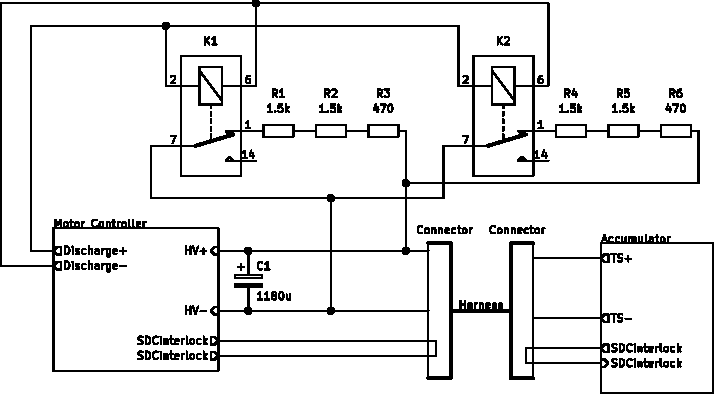
\includegraphics[width=0.7\textwidth]{./img/MC_discharge.pdf}
	\caption{Discharge circuit.}
	\label{fig:discharge-circuit}
\end{figure}

\ref{fig:discharge-circuit} shows a simplified connection of a discharge resistors. Discharge resistors are placed in \glspl{mc} right next to the only capacity that provides a storage for potentially dangerous charge/energy. If \gls{hv} cable is disconnected on either side, the \gls{sdc} opens due to the interlocks and both \glspl{air} open. Because there is no output capacitance in \gls{acp} there is no way the power could be on \gls{acp} output \gls{hv} connector.

Sum of capacity of all capacitors in \glspl{mc} is 2360 uF. For discharging this capacity in less than 5 seconds to voltage (below 60V), maximum resistor value is calculated by solving R from \ref{eq:discharge_voltage}.

\begin{equation}
	V_{c}=V_{s}*e^{(\frac{-t}{R*C})}
	\label{eq:discharge_voltage}
\end{equation}

\paragraph{Values}
\begin{itemize}
	\item $V_c = 60 V$ (safe voltage limit)
	\item $V_s = 403.2 V$ (TS voltage)
	\item $t = 5 s$ (maximal discharge time)
	\item $C = 2360\mu$F (total capacity in TS)
\end{itemize}

Maximal resistance from \ref{eq:discharge_voltage} resulting $R = 1112\Omega$ is for total capacity on \gls{ts}. In out case, capacity is split between two \glspl{mc}. Two parallel resistor combinations of two 1.5k$\Omega$ and one 470$\Omega$ resistors in series in each \gls{mc} is used. (4 in total). 1.5k$\Omega$ resistors are THS151K5J. 470$\Omega$ resistors are \todo[inline]{add resistor type}. Total value of Discharge Resistor Bank is $R = 867.5\Omega$, which is less than $R = 1112\Omega$. The 60V threshold with this configuration is reached in 3.9s. \ref{fig:discharge_voltage_time} shows TS voltage in time during discharging.

\begin{figure}
	\begin{tikzpicture}
		\begin{axis}[
			use units,
			x unit=s,
			y unit=V,
			xlabel=time,
			ylabel=voltage,
			width=0.9\textwidth,
			height=0.5\textwidth,
			grid=major,
			xmin=0,
			ymin=0,
			xmax=20
			]
			\addplot[red, smooth] table[
				x=time,
				y=voltage,
				col sep=comma
				] {./data/TS_discharge_voltage.csv}; 
		\end{axis}
	\end{tikzpicture}
	\caption{Discharge voltage on resistor vs. time}
	\label{fig:discharge_voltage_time}
\end{figure}


\begin{figure}
	\begin{tikzpicture}
		\begin{axis}[
			use units,
			x unit=s,
			y unit=A,
			xlabel=time,
			ylabel=current,
			width=0.9\textwidth,
			height=0.5\textwidth,
			grid=major,
			xmin=0,
			ymin=0,
			xmax=20
			]
			\addplot[red, smooth] table[
			x=time,
			y=current,
			col sep=comma
			] {./data/TS_discharge_current.csv}; 
		\end{axis}
	\end{tikzpicture}
	\caption{Discharge current through resistors vs. time}
	\label{fig:discharge_current_time}
\end{figure}



The formula describing \ref{fig:discharge_current_time} is:

\begin{equation}
	I_{d}=\frac{V_{c}}{R_{d}}	
\end{equation}

\begin{equation}
	I_{d}=\frac{V_{s}*e^{(\frac{-t}{R*C})}}{R_{d}}
	\label{eq:discharge_current}
\end{equation}

Where $Vs$ is voltage on \gls{ts}, $Rd$ is total value of discharge resistor banks and $Id$ is sum of current  going through all resistor banks. Current through individual resistor banks can be calculated as $I_{d}$/$4$.


\begin{figure}
	\begin{tikzpicture}
		\begin{axis}[
			use units,
			x unit=s,
			y unit=W,
			xlabel=time,
			ylabel=power loss,
			width=0.9\textwidth,
			height=0.5\textwidth,
			grid=major,
			xmin=0,
			ymin=0,
			xmax=20
			]
			%\pgfplotstableread{./data/TS_discharge_current.csv}\dischargeData;
			\addplot[red, smooth] table[
				x=time,
				y expr=(\thisrow{current}/4)^2*867.5*4,
				col sep=comma
				] {./data/TS_discharge_current.csv}; 
			\addlegendentry{whole resistor bank $P_{loss}$}
			\addplot[orange, smooth] table[
				x=time,
				y expr=(\thisrow{current}/4)^2*1500,
				col sep=comma
				] {./data/TS_discharge_current.csv};
			\addlegendentry{$1.5k\Omega$ resistor bank $P_{loss}$}
			\addplot[blue, smooth] table[
				x=time,
				y expr=(\thisrow{current}/4)^2*470,
				col sep=comma
				] {./data/TS_discharge_current.csv};
			\addlegendentry{$470\Omega$ resistor bank $P_{loss}$}
		\end{axis}
	\end{tikzpicture}
	\caption{Discharge power loss on 1 bank and individual resistors vs. time}
	\label{fig:discharge_power_time}
\end{figure}

Peak power is 15 W and the resistor can handle this power over 20 s, see \ref{app:discharge-resistor_1k5_sheet}.

\begin{table}[H]
	\centering
	\caption{General data of the discharge circuit}
	\begin{tabularx}{\textwidth}{|X|X|}
		\hline
		Resistor Type: & wirewound power resistor \\[\TableSize]
		\hline
		Resistance: & 867.5$\Omega$ \\[\TableSize]
		\hline
		Continuous power rating: & 15W \\[\TableSize]
		\hline
		Overload power rating (1 sec): & \\[\TableSize]
		\hline
		Overload power rating (5 sec): &  \\[\TableSize]
		\hline
		Overload power rating (15 sec): &  \\[\TableSize]
		\hline
		Voltage rating: & 265V (2 in series result in ~530V) \\[\TableSize]
		\hline
		Maximum expected current: & 0.4A current total (0.1A per resistor bank, 4 in series) \\[\TableSize]
		\hline
		Average current: & 0.04A on resistor(taking account 4 seconds of discharging) \\[\TableSize]
		\hline
		Cross-sectional area of the wire used: & $0.129 mm^2$ \\[\TableSize]
		\hline
	\end{tabularx}%
	\label{tab:dischrage-circ}%
\end{table}%

\begin{table}[H]
	\centering
	\caption{General data of the dis-charge relay}
	\begin{tabularx}{\textwidth}{|X|X|}
		\hline
		Relay Type: & mechanical, DC \\[\TableSize]
		\hline
		Contact arrangement: & 1 pole, normally closed  \\[\TableSize]
		\hline
		Continuous DC current:  & \textbf{??}  \\[\TableSize]
		\hline
		Voltage rating  & \textbf{??}\\[\TableSize]
		\hline
		Nominal Coil Voltage: & \textbf{??}\\[\TableSize]
		\hline
		FET type: & \textbf{??} \\[\TableSize]
		\hline
		Maximum Drain-Source Current: & \textbf{??}  \\[\TableSize]
		\hline
		Drain-Source Breakdown Voltage: & \textbf{??}  \\[\TableSize]
		\hline
		On Characteristics Gate Threshold Voltage: & \textbf{??} \\[\TableSize]
		\hline
		Cross-sectional area of the wire used: & \textbf{??} \\[\TableSize]
		\hline
	\end{tabularx}%
	\label{tab:discharge-relay}%
\end{table}%


\subsubsection{Position in car}
%Provide CAD-renderings showing all relevant parts. Mark the parts in the rendering, if necessary.

Discharge resistors are mounted on aluminum cooler also with IGBT modules in \gls{mc} boxes.